\documentclass{article}

%% doc settings
\hyphenchar\font=-1 % suppress hyphenation
\setlength\parindent{0pt} % suppress indentation
\usepackage[margin=1.25truein]{geometry} % set page margins

%% libraries 
\usepackage{listings}
\usepackage{fancyhdr}
\usepackage{lastpage}
\usepackage{url}
\usepackage{xcolor}
\usepackage{hyperref}
\usepackage{amssymb}
\usepackage{amsthm}
\usepackage{amsmath}
\usepackage{algorithm}
\usepackage{algcompatible}
\usepackage{natbib}
\usepackage{tikz}
\usepackage{pgfplots}
\usepackage{textcomp}
\usepackage{subcaption}
\usetikzlibrary{shapes, arrows}

%% link viz
\hypersetup{
    colorlinks = true,
    linkcolor = red,
    urlcolor = red,
    citecolor = black
}

%% code colors 
\definecolor{codegreen}{rgb}{0,0.6,0}
\definecolor{codegray}{rgb}{0.5,0.5,0.5}
\definecolor{codepurple}{rgb}{0.58,0,0.82}
\definecolor{backcolour}{rgb}{0.95,0.95,0.92}

\lstdefinestyle{mystyle}{
    backgroundcolor=\color{backcolour},   
    commentstyle=\color{codegreen},
    keywordstyle=\color{magenta},
    numberstyle=\tiny\color{codegray},
    stringstyle=\color{codepurple},
    basicstyle=\ttfamily\footnotesize,
    breakatwhitespace=false,         
    breaklines=true,                 
    captionpos=b,                    
    keepspaces=true,                 
    numbers=left,                    
    numbersep=5pt,                  
    showspaces=false,                
    showstringspaces=false,
    showtabs=false,                  
    tabsize=2
}

\lstset{style=mystyle}

%% math ops
\DeclareMathOperator*{\argmax}{argmax} % thin space, limits underneath in displays

%% page nums
\pagestyle{fancy}
\fancyhf{}
\fancyfoot[C]{Pg. \thepage \space of \pageref*{LastPage}}
\renewcommand{\headrulewidth}{0pt}

%% begin doc
\begin{document}
\title{SYSEN 5200: Systems Analysis Behavior and Optimization\\~\\
    \Large Monte Carlo Simulation
}
\author{
    Nick Kunz [NetID: \url{nhk37}] \hyperlink{nhk37@cornell.edu}{nhk37@cornell.edu}}
\date{March 6, 2023}
\maketitle
\thispagestyle{fancy}

%% body doc
\begin{enumerate}

    \item Suppose that you want to generate a random sample from a p.d.f. with the following distribution:

    \begin{equation}
        \begin{split}
            f(x) &= \begin{cases}
                \frac{3x^{2}}{8} & \text{ for } 0 \leq x \leq 2\\
                0 & \text{otherwise}
            \end{cases}
        \end{split}
    \end{equation}

    the equivalent c.d.f can be derived as:
    \begin{equation}
        \begin{split}
            F(x) &= \int_{-\infty}^{x} f(t)\, dt\\
            &= \int_{0}^{x} \frac{3t^{2}}{8}\, dt\\
            &= \frac{t^{3}}{8}\Big|_{0}^{x}\\
            &= \frac{x^{3}}{8}
        \end{split}
    \end{equation}

    Therefore, we have:
    \begin{equation}
        F(x) = \begin{cases}
        0 & \text{for } x<0 \\
        \frac{x^{3}}{8} & \text{for } 0 \leq x \leq 2 \\
        1 & \text{for } x>2
    \end{cases}
    \end{equation}

    when inverted is:

    \begin{equation}
        F^{-1}(y) = \begin{cases}
        0 & \text{for } y \leq 0 \\
        \sqrt[3]{8y} & \text{for } 0 < y \leq 1 \\              
        2 & \text{for } y > 1
        \end{cases}
        \end{equation}\\

    where $g(y) = F^{-1}(y)$ that recovers the r.v. $X$ with the desired p.d.f. $f(x)$ from $Y \sim U[0,1].

\newpage

    \item Suppose that the lifetime of each component $i$ is independent and follows a distribution that is the maximum of zero and a normal random variable with mean $\mu_i$ and standard deviation $\sigma_i$ (both in minutes), whose values are given by: $\mu_1 = 60, \sigma_1 = 15; \mu_2 = 50, \sigma_2 = 10; \mu_3 = 75, \sigma_3 = 15; \mu_4 = 75, \sigma_4= 20; \mu_5 = 60, \sigma_5 = 15; \mu_6 = 70, \sigma_6 = 15$.
    
    \begin{enumerate}
        \item Considering the structure function of the following system:
        \begin{equation}
            \phi(x) = \min(\max(\min(x_1, x_2), x_3), x_4, \max(x_5, x_6))
        \end{equation}
    
        \item A simulation was conducted with over 1,000 replications to estimate the probability that the system will be functional for more than 60 minutes with a 95\% confidence interval.
    
\begin{lstlisting}[language=Python, title=Fig. Python 2(b)]
## libraries
import numpy as np

## structure func
def phi(x):
    return min(max(min(x[0], x[1]), x[2]), x[3], max(x[4], x[5]))

## simulation
def simulate():
    x = np.maximum(0, np.random.normal(
        [60, 50, 75, 75, 60, 70], ## mu
        [15, 10, 15, 20, 15, 15] ## sigma
        )
    )
    return phi(x) > 60

## compute
n = 1001
results = [simulate() for i in range(n)]
prob = sum(results) / n
lower = prob - 1.96 * np.sqrt(prob * (1 - prob) / n)
upper = prob + 1.96 * np.sqrt(prob * (1 - prob) / n)

## results 
print(f"Probability: {prob:.4f}")
print(f"95% CI: ({lower:.4f}, {upper:.4f})")
\end{lstlisting}
    
    Probability: \textbf{0.5834}\\
    95\% CI: \textbf{(0.5529, 0.6140)}\\

    \item Suppose that the error of the estimate is to be bounded by 0.01 with 0.95 probability. Using Chebyshev’s inequality, we estimate the number of replications is sufficient to provide this guarantee as:
    \begin{equation}
        \begin{split}
            P(|\hat{p}-p| \geq 0.01) \leq \frac{Var(\hat{p})}{0.01^2} &= \frac{p(1-p)/n}{0.01^2}\\
n &\geq \frac{p(1-p)}{(0.01^2 \cdot 0.05)}\\
n &\geq \frac{0.5 \cdot 0.5}{(0.01^2 \cdot 0.05)} = 50,000
        \end{split} 
    \end{equation}

    Assuming that the approximation from Central Limit Theorem holds, we have:
    \begin{equation}
        \begin{split}
          n \geq \left(\frac{z_\alpha/2^\sigma}{E}\right)^2 = \left(\frac{1.96}{0.01}\right)^2 \cdot 0.5 \cdot 0.5 \approx 9,604.
        \end{split}
    \end{equation}
    
\item Another simulation was conducted with over 1,000 replications to estimate the expected lifetime of the system in minutes with a 95\% confidence interval.
    
\begin{lstlisting}[language=Python, title=Fig. Python 2(d)]
## libraries
import numpy as np

## structure func
def phi(x):
    return min(max(min(x[0], x[1]), x[2]), x[3], max(x[4], x[5]))

## simulation
def simulate():
    x = np.maximum(0, np.random.normal(
        [60, 50, 75, 75, 60, 70], ## mu
        [15, 10, 15, 20, 15, 15] ## sigma
        )
    )
    return phi(x)

## compute 
n = 1001
results = [simulate() for i in range(n)]
mean = np.mean(results)
lower = mean - 1.96 * np.std(results, ddof=1) / np.sqrt(n)
upper = mean + 1.96 * np.std(results, ddof=1) / np.sqrt(n)

## results 
print(f"Expected L: {mean:.2f} minutes")
print(f"95% CI: ({lower:.2f}, {upper:.2f}) minutes")
\end{lstlisting}

    Expected L: \textbf{61.80} min.\\
    95\% CI: \textbf{(61.05, 62.56)} min.\\

    \item Suppose that the error of the estimate is to be bounded by 1 minute with 0.95 probability. Using Chebyshev’s inequality, we estimate the number of replications is sufficient to provide this guarantee as:
    \begin{equation}
        \begin{split}
            n \geq \frac{\sigma_1^2+\sigma_2^2+\sigma_3^2+\sigma_4^2+\sigma_5^2+\sigma_6^2}{0.05} = \frac{15^2+10^2+15^2+20^2+15^2+15^2}{0.05} = 2,843
        \end{split}
    \end{equation}

    Assuming that the approximation from Central Limit Theorem holds, we have:
    \begin{equation}
        \begin{split}
            n \geq \left(\frac{z_{\alpha/2}\sigma}{E}\right)^2 =  \left(\frac{1.96\cdot 18.8}{1}\right)^2 \approx 546
        \end{split}
    \end{equation}
                
\end{enumerate}

\newpage
    \item One application of Monte Carlo Simulation is estimating a difficult to evaluate integral. Here we will perform a simple simulation to estimate the area of a unit circle.

    \begin{enumerate}
        \item First we will generate 10,000 points uniformly on $U[-1, 1]$ using 50 uniform-sized bins.\\

\begin{lstlisting}[language=Python, title=Fig. Python 3(a)]
## libraries
import numpy as np
import matplotlib.pyplot as plt

## replicate
X = np.random.uniform(-1, 1, 10_000)

## plot
plt.hist(
    x = X, 
    bins = 50, 
    density = True
)

## plot labels
plt.xlabel('Value')
plt.ylabel('Frequency')

## plot preview
plt.show()\end{lstlisting}
            
\begin{align*}
    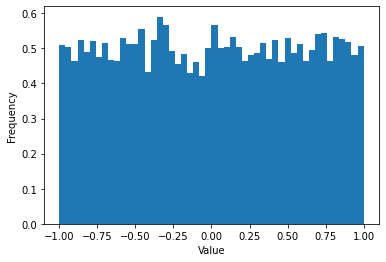
\includegraphics[width=0.6\textwidth]{uni.png}
\end{align*}

\newpage
        \item Then we generate 10,000 points uniformly distributed in a square around the origin with corners (-1,-1), (-1,1), (1,-1), and (1,1). We independently generate the $X$ and $Y$-coordinates of a point to be $U[-1, 1]$. Then we create an additional array $Z$ of length 10,000, which indicates whether each random point lies within a circle of radius 1 centered at the origin.\\

\begin{lstlisting}[language=Python, title=Fig. Python 3(b)]
## libraries
import numpy as np
import matplotlib.pyplot as plt

## replicate
X = np.random.uniform(-1, 1, 10_000)
Y = np.random.uniform(-1, 1, 10_000)

## compute distance
R = np.sqrt(X**2 + Y**2)
Z = np.where(R <= 1, 1, 0)

## plot
fig, ax = plt.subplots(figsize=(5, 5))
ax.scatter(
    x = X, 
    y = Y, 
    c = Z, 
    s = 2.0,
    cmap = plt.cm.Paired
)

## plot labels
ax.set_xlabel('X')
ax.set_ylabel('Y')
ax.set_aspect('equal')

## plot preview
plt.show()
\end{lstlisting}
            
\begin{align*}
    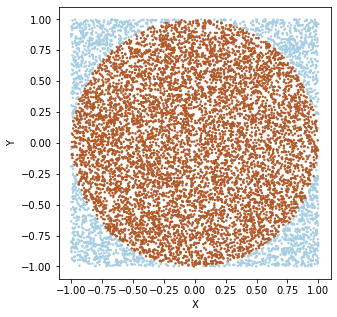
\includegraphics[width=0.5\textwidth]{pi.png}
\end{align*}

\newpage
        \item Given $n$ random points above, we can estimate $\pi$ as $\hat{\pi_n} = 4 N_{circle}/n$, where $N_{circle}$ is the number of random points which lie within the circle. For $n$ between 1 and 1000, we plot the relative error $|\pi_n - \pi| / \pi$, as well as the function $1/\sqrt{n}$.
        
\begin{lstlisting}[language=Python, title=Fig. Python 3(c)]
## libraries
import numpy as np
import matplotlib.pyplot as plt

## pi
pi_true = np.pi

## number of replications
ns = np.arange(1, 1001)

## initialize estimations of pi and errors
pi_est = np.zeros_like(ns, dtype = float)
rel_err = np.zeros_like(ns, dtype = float)

## replications and estimations
for i, n in enumerate(ns):
    X = np.random.uniform(-1, 1, n)
    Y = np.random.uniform(-1, 1, n)

    ## compute distances
    R = np.sqrt(X**2 + Y**2)
    N_circle = np.count_nonzero(R <= 1)

    ## estimate pi and compute error
    pi_est[i] = 4 * N_circle / n
    rel_err[i] = np.abs(pi_est[i] - pi_true) / pi_true

## plot
fig, ax = plt.subplots()
ax.scatter(ns, rel_err, label = 'Relative Error', alpha = 0.5, s = 5)
ax.plot(ns, 1/np.sqrt(ns), label = '1 / sqrt(n)', color = 'orange')

## plot labels
ax.set_xlabel('n')
ax.set_ylabel('Relative Error')
ax.legend()

## plot preview
plt.show()
\end{lstlisting}
\begin{align*}
    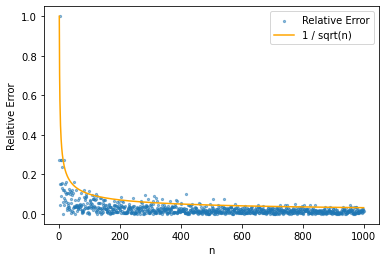
\includegraphics[width=0.55\textwidth]{err.png}
\end{align*}

    \end{enumerate}
    
%% end
\end{enumerate}
\end{document}